%        File: arfc-beamer.tex
%     Created: Sun May 5 10:00 PM 2013 C
%


%\documentclass[11pt,handout]{beamer}
\documentclass[9pt]{beamer}
\usetheme[white]{Illinois}
%\title[short title]{long title}
\title[Spent Fuel]{International Spent Nuclear Fuel Options}

%\subtitle[short subtitle]{long subtitle}
\subtitle[NNSA Seminar]{Argonne Nuclear Nonproliferation Seminar:\\Reactors 
and the Commercial Nuclear Industry}
%\author[short name]{long name}
\author[K. Huff]{Kathryn Huff\\Advanced Reactors and Fuel Cycles Group}
%\date[short date]{long date}
\date[09.21.2017]{September 21, 2017}
%\institution[short name]{long name}
\institute[UIUC]{University of Illinois at Urbana-Champaign}

%\usepackage{bbding}
\usepackage{amsfonts}
\usepackage{amsmath}
\usepackage{xspace}
\usepackage{graphicx}
\usepackage{subfigure}
\usepackage{booktabs} % nice rules for tables
\usepackage{microtype} % if using PDF
\usepackage{bigints}
\usepackage{minted}

\newcommand{\units}[1] {\:\text{#1}}%
\newcommand{\SN}{S$_N$}%{S$_\text{N}$}%{$S_N$}%
\DeclareMathOperator{\erf}{erf}
%I need some complimentary error funcitons... 
\DeclareMathOperator{\erfc}{erfc}
%page numbers
\setbeamertemplate{footline}[page number]
\setbeamertemplate{caption}[numbered]
%Those icons in the references are terrible looking
\setbeamertemplate{bibliography item}[text]

%%%% Acronym support

\usepackage[acronym,toc]{glossaries}
\include{acros}

\makeglossaries

%try to get rid of header on title page\dots
\makeatletter
    \newenvironment{withoutheadline}{
        \setbeamertemplate{headline}[default]
        \def\beamer@entrycode{\vspace*{-\headheight}}
    }{}
\makeatother

\begin{document}
%%%%%%%%%%%%%%%%%%%%%%%%%%%%%%%%%%%%%%%%%%%%%%%%%%%%%%%%%%%%%
%% From uw-beamer Here's a handy bit of code to place at 
%% the beginning of your presentation (after \begin{document}):
\newcommand*{\alphabet}{ABCDEFGHIJKLMNOPQRSTUVWXYZabcdefghijklmnopqrstuvwxyz}
\newlength{\highlightheight}
\newlength{\highlightdepth}
\newlength{\highlightmargin}
\setlength{\highlightmargin}{2pt}
\settoheight{\highlightheight}{\alphabet}
\settodepth{\highlightdepth}{\alphabet}
\addtolength{\highlightheight}{\highlightmargin}
\addtolength{\highlightdepth}{\highlightmargin}
\addtolength{\highlightheight}{\highlightdepth}
\newcommand*{\Highlight}{\rlap{\textcolor{HighlightBackground}{\rule[-\highlightdepth]{\linewidth}{\highlightheight}}}}
%%%%%%%%%%%%%%%%%%%%%%%%%%%%%%%%%%%%%%%%%%%%%%%%%%%%%%%%%%%%%
%%--------------------------------%%
\begin{withoutheadline}
\frame{
  \titlepage
}
\end{withoutheadline}

%%--------------------------------%%
\AtBeginSection[]{
\begin{frame}
  \frametitle{Outline}
  \tableofcontents[currentsection]
\end{frame}
}

\section{Introduction}
\subsection{Nuclear Nations}

\begin{frame}
  \frametitle{Nuclear Power Nations}
  % a comment
  \begin{figure}[htbp!]
    \begin{center}
      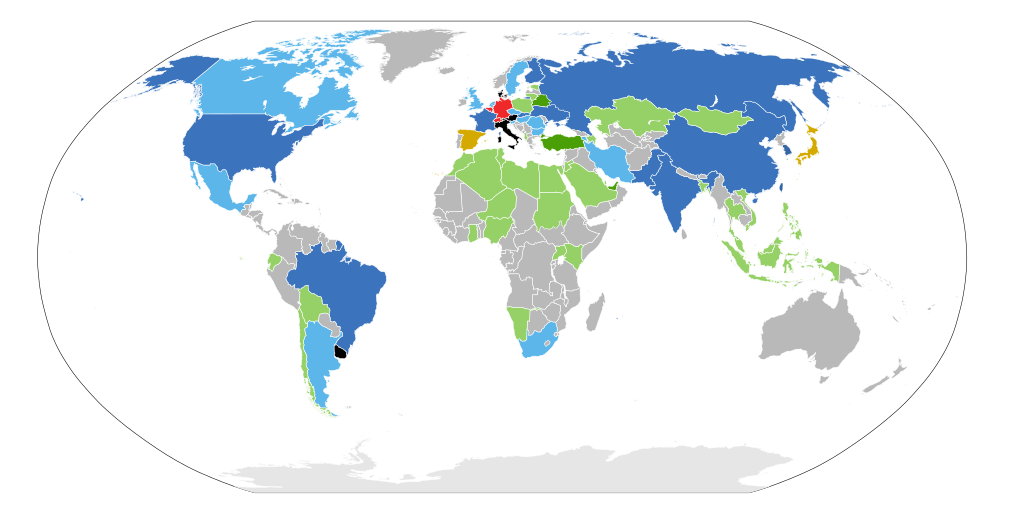
\includegraphics[width=\textwidth]{./images/nuclear-nations-map.png}\\

\vspace{-10mm}
      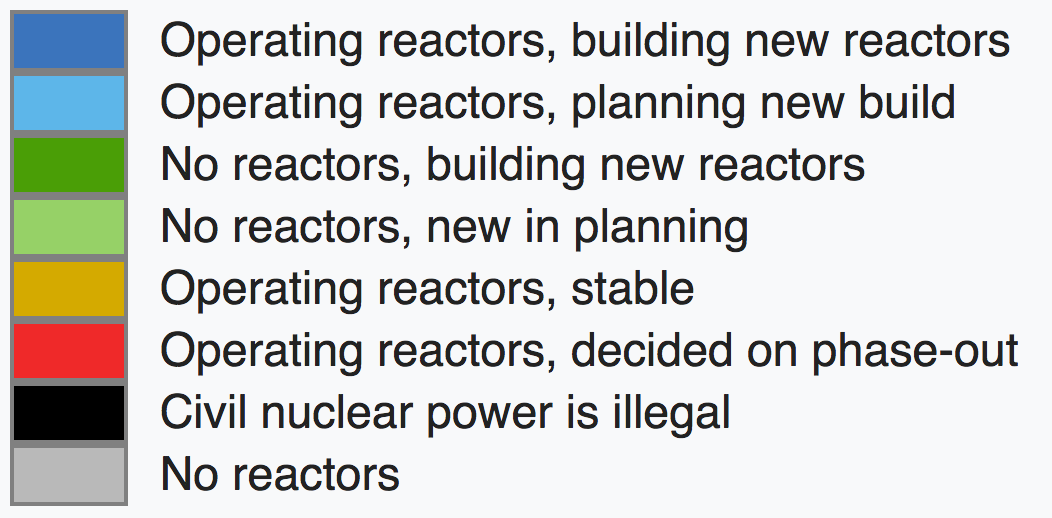
\includegraphics[height=0.2\textheight]{./images/nuclear-nations-legend.png}
    \end{center}
          \caption{Nuclear power status of all nations 
          \cite{paleogene_file:nuclear_2017}.}
    \label{fig:nuc-nations-map}
  \end{figure}
\end{frame}

\begin{frame}
  \frametitle{Nuclear Weapons Nations}
  % a comment
  \begin{figure}[htbp!]
    \begin{center}
      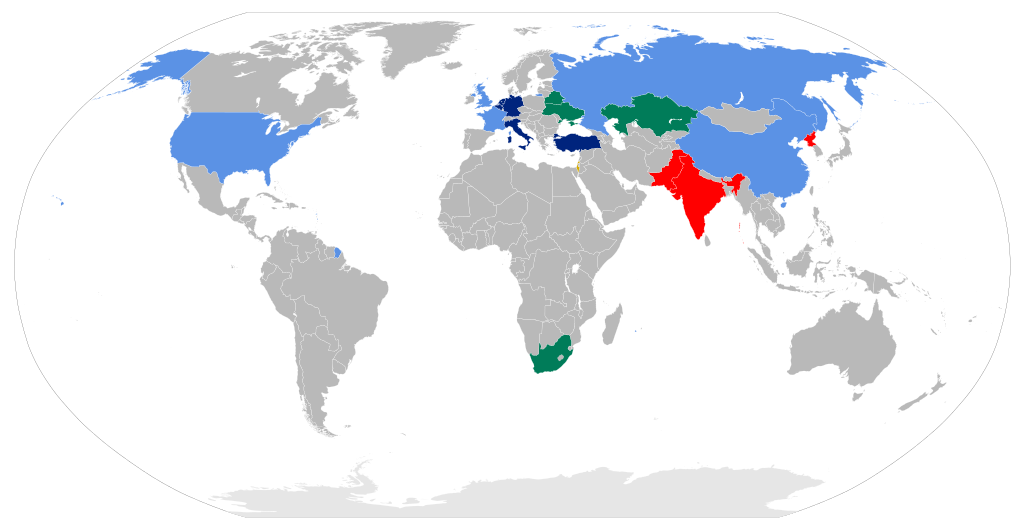
\includegraphics[width=\textwidth]{./images/nuclear-weapons-map.png}\\

\vspace{-10mm}
      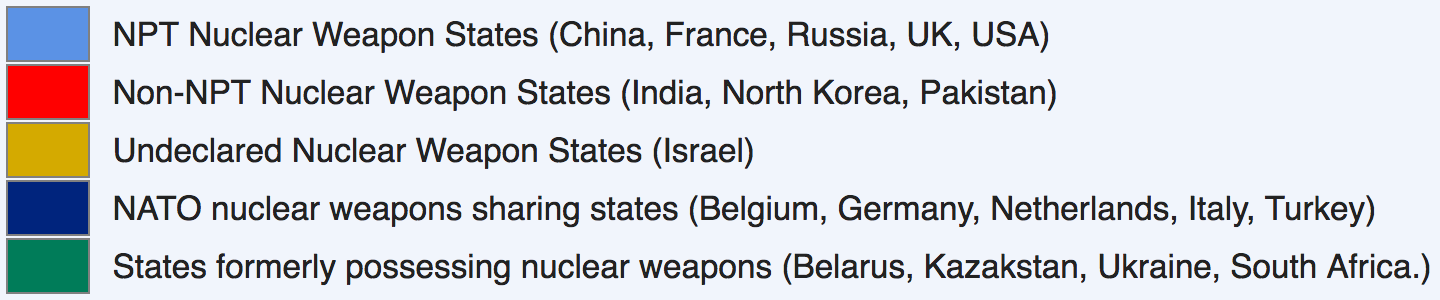
\includegraphics[height=0.2\textheight]{./images/nuclear-weapons-legend.png}
    \end{center}
          \caption{Nuclear power status of all nations 
          \cite{paleogene_file:nuclear_2017}.}
    \label{fig:nuc-nations-map}
  \end{figure}
\end{frame}




\begin{frame}
  \frametitle{Power vs. Weapons}
  % a comment
        \begin{columns}
                \column[t]{0.6\textwidth}
        \begin{center}
      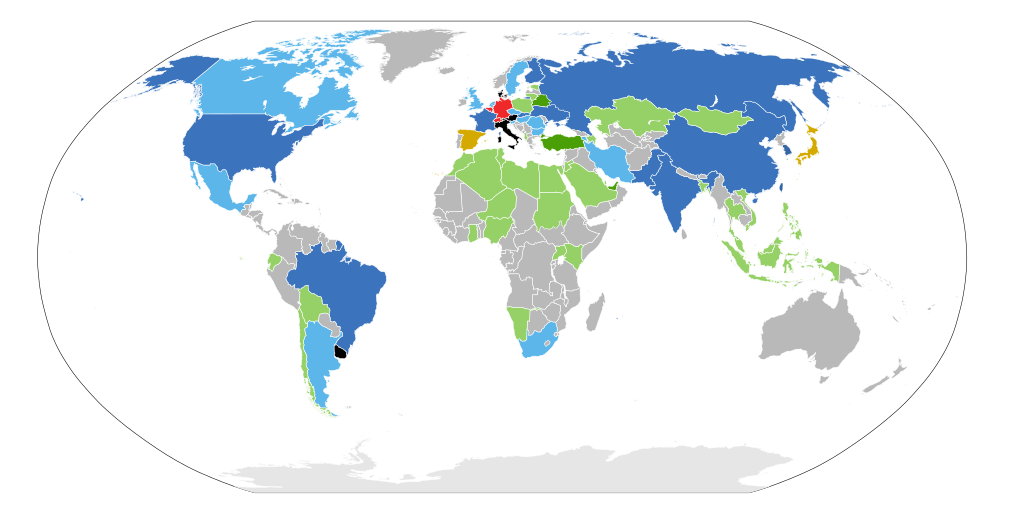
\includegraphics[width=\textwidth]{./images/nuclear-nations-map.png}\\
    \end{center}
                \column[t]{0.6\textwidth}
\hspace{-1in}
                \begin{center}
		      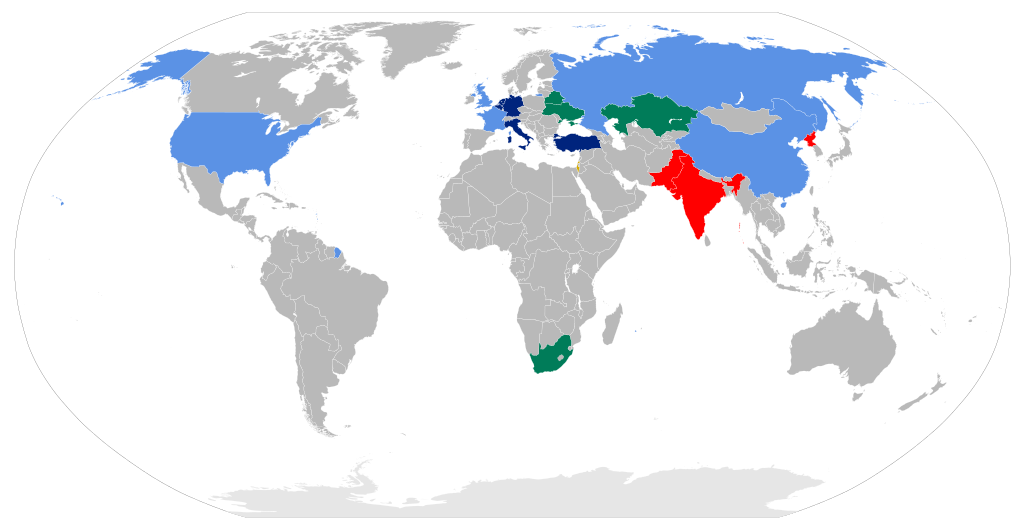
\includegraphics[width=\textwidth]{./images/nuclear-weapons-map.png}
                \end{center}
        \end{columns}
\end{frame}        

\begin{frame}
  \frametitle{International Reactors}
  % a comment
  \begin{figure}[htbp!]
    \begin{center}
      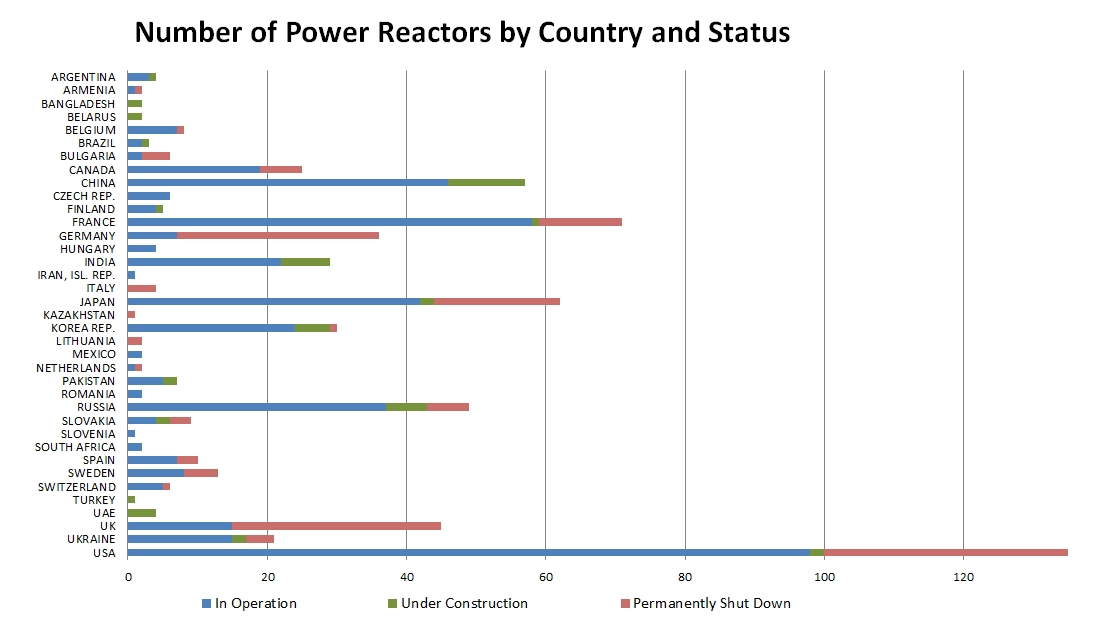
\includegraphics[width=\textwidth]{./images/nuclear-nations.eps}
    \end{center}
          \caption{Nuclear reactors internationally, replicated from 
          \cite{iaea_country_2015}.}
    \label{fig:nuc-nations}
  \end{figure}
\end{frame}

\begin{frame}
  \frametitle{Nuclear Capacity}
  \begin{figure}[htbp!]
    \begin{center}
      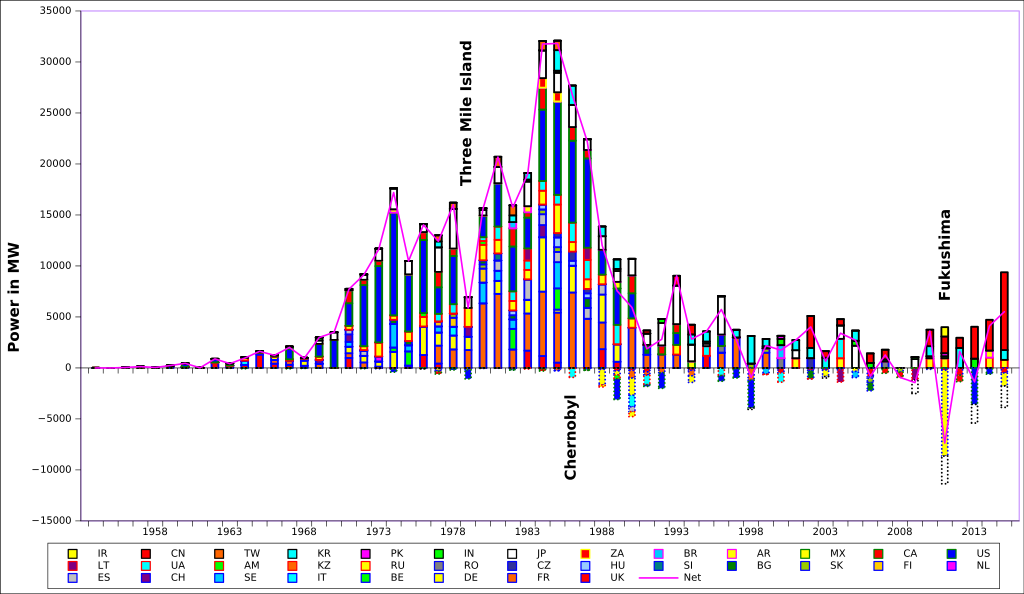
\includegraphics[width=0.9\textwidth]{./images/nuclear-nations-deployments.png}
    \end{center}
          \caption{Nuclear power deployments as a function of time
          \cite{torsch_global_2013}.}
    \label{fig:nuc-nations-deployments}
\end{figure}
\end{frame}


\subsection{Spent Fuel Options}

%%--------------------------------%%
\begin{frame}[c]
    \frametitle{Array of Possible Options}
    \begin{figure}[htbp!]
  \begin{center}
    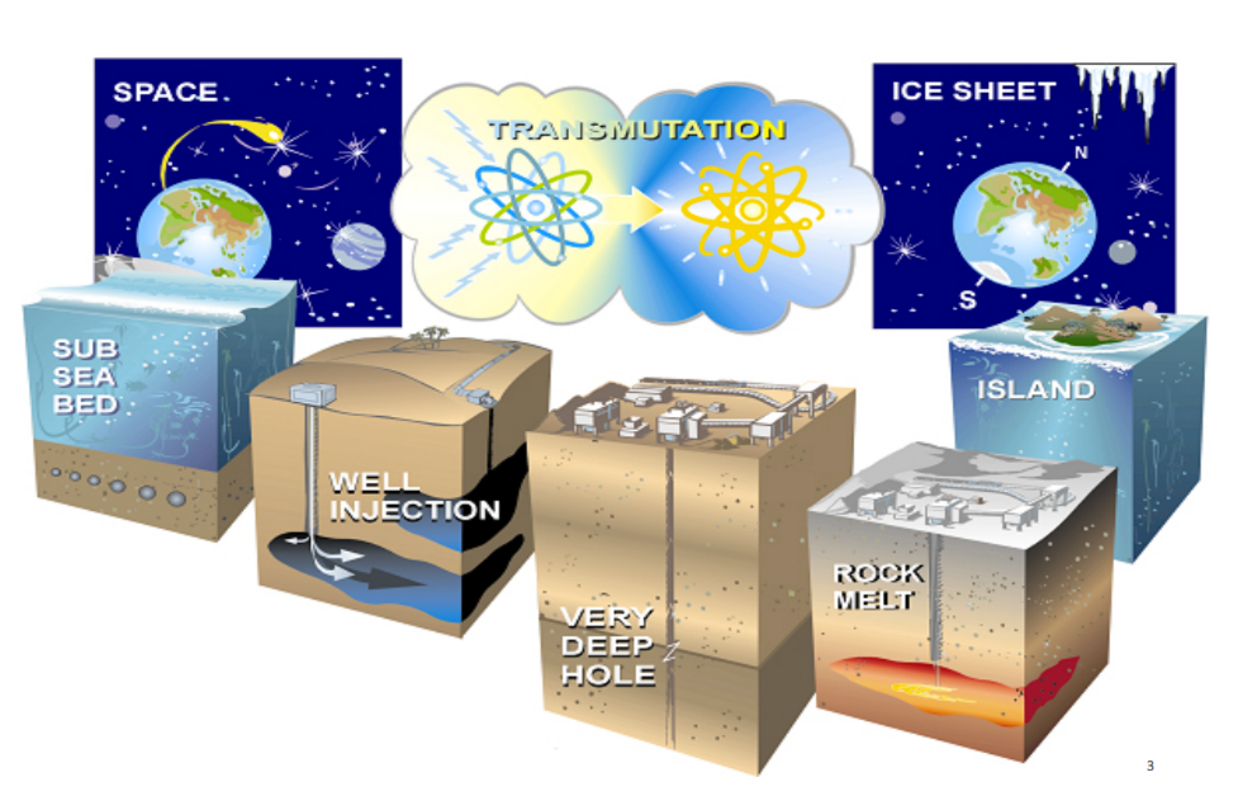
\includegraphics[height=0.7\textheight]{./images/alternative_options.eps}
  \end{center}
  \caption{An array of options have been considered in the past 
    \cite{peters_whats_2013}.}
  \label{fig:alternative_options}
\end{figure}

  \end{frame}

\subsection{Repository Concepts}
% layouts
% EBS choices
% Geologies


\begin{frame}[c]
  \frametitle{Clay Disposal Environments}

  \begin{figure}[h!]
    \begin{center}
      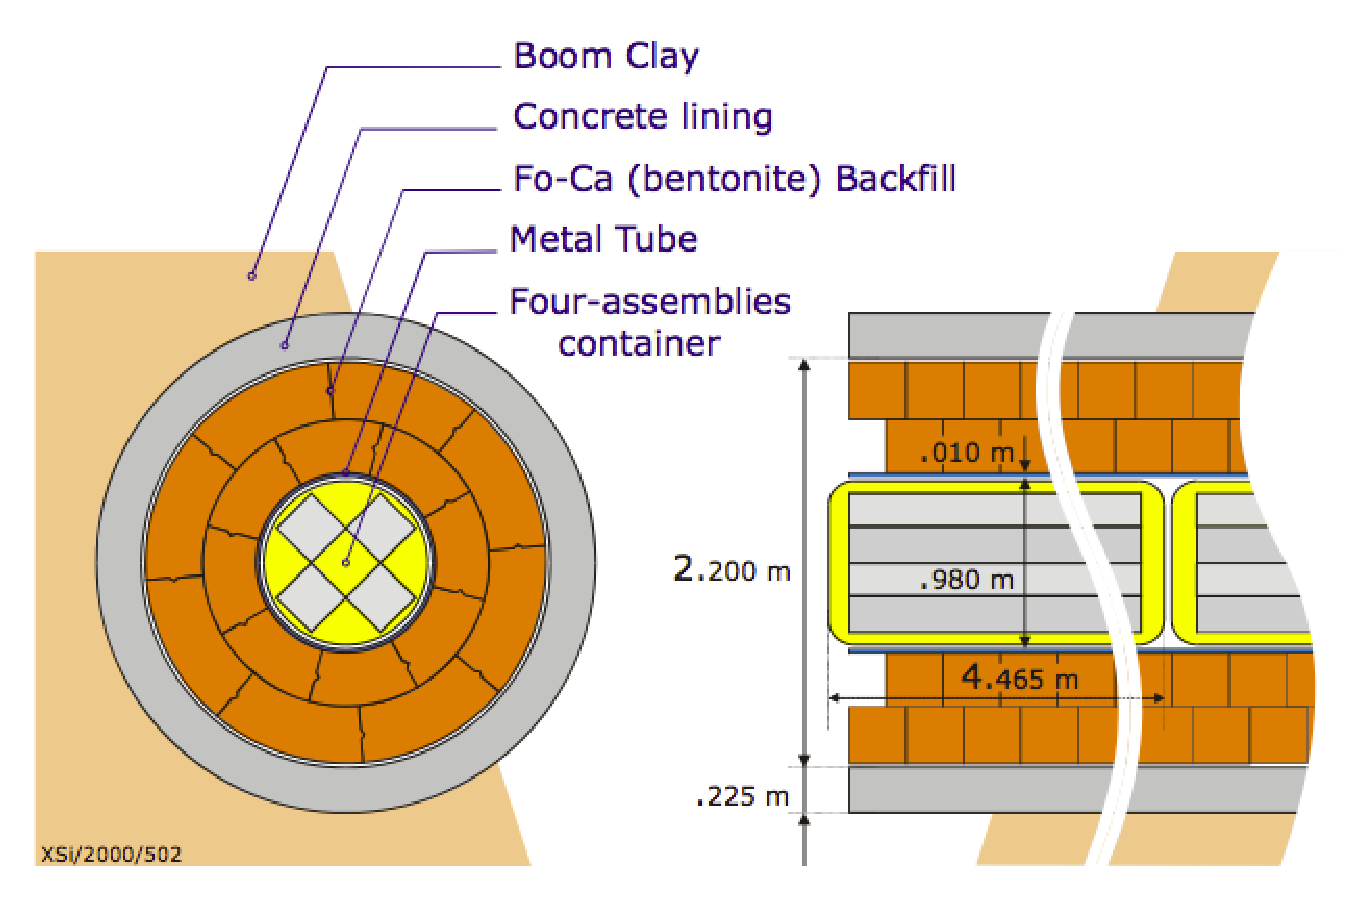
\includegraphics[height=.7\textheight]{./images/belgianClayRedImp.eps}
    \end{center}
    \caption{Belgian reference concept in Boom Clay 
    \cite{von_lensa_red-impact_2008}.}
    \label{fig:belgianClayRedImp}
  \end{figure}

\end{frame}

\begin{frame}[c]
  \frametitle{Granite Disposal Environments}

  \begin{figure}[h!]
    \begin{center}
      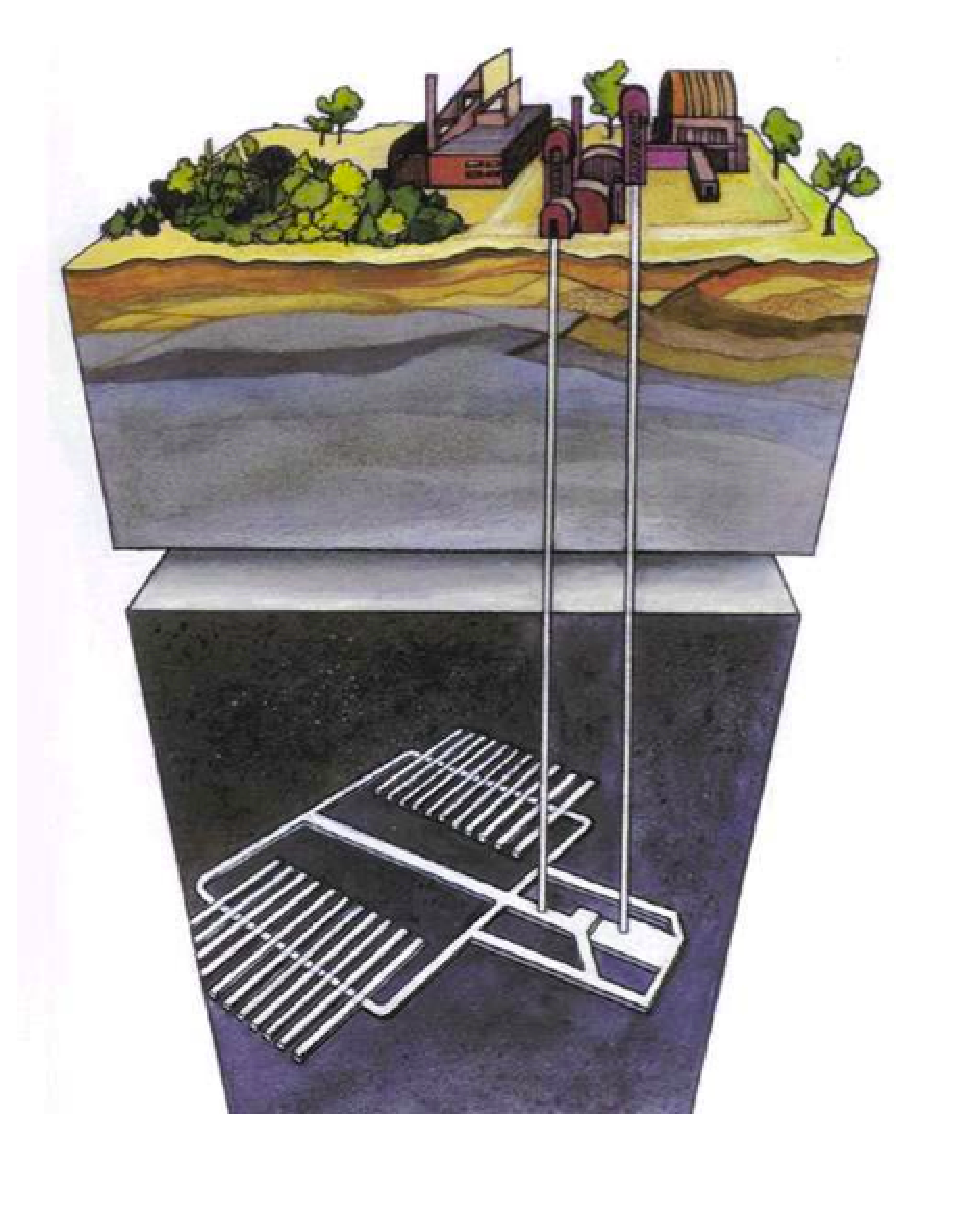
\includegraphics[height=.7\textheight]{./images/czechGraniteRedImp.eps}
    \end{center}
    \caption{Czech reference concept in Granite 
    \cite{von_lensa_red-impact_2008}.}
    \label{fig:czechGraniteRedImp}
  \end{figure}

\end{frame}

\begin{frame}[c]
  \frametitle{Salt Disposal Environments}

  \begin{figure}[h!]
    \begin{center}
      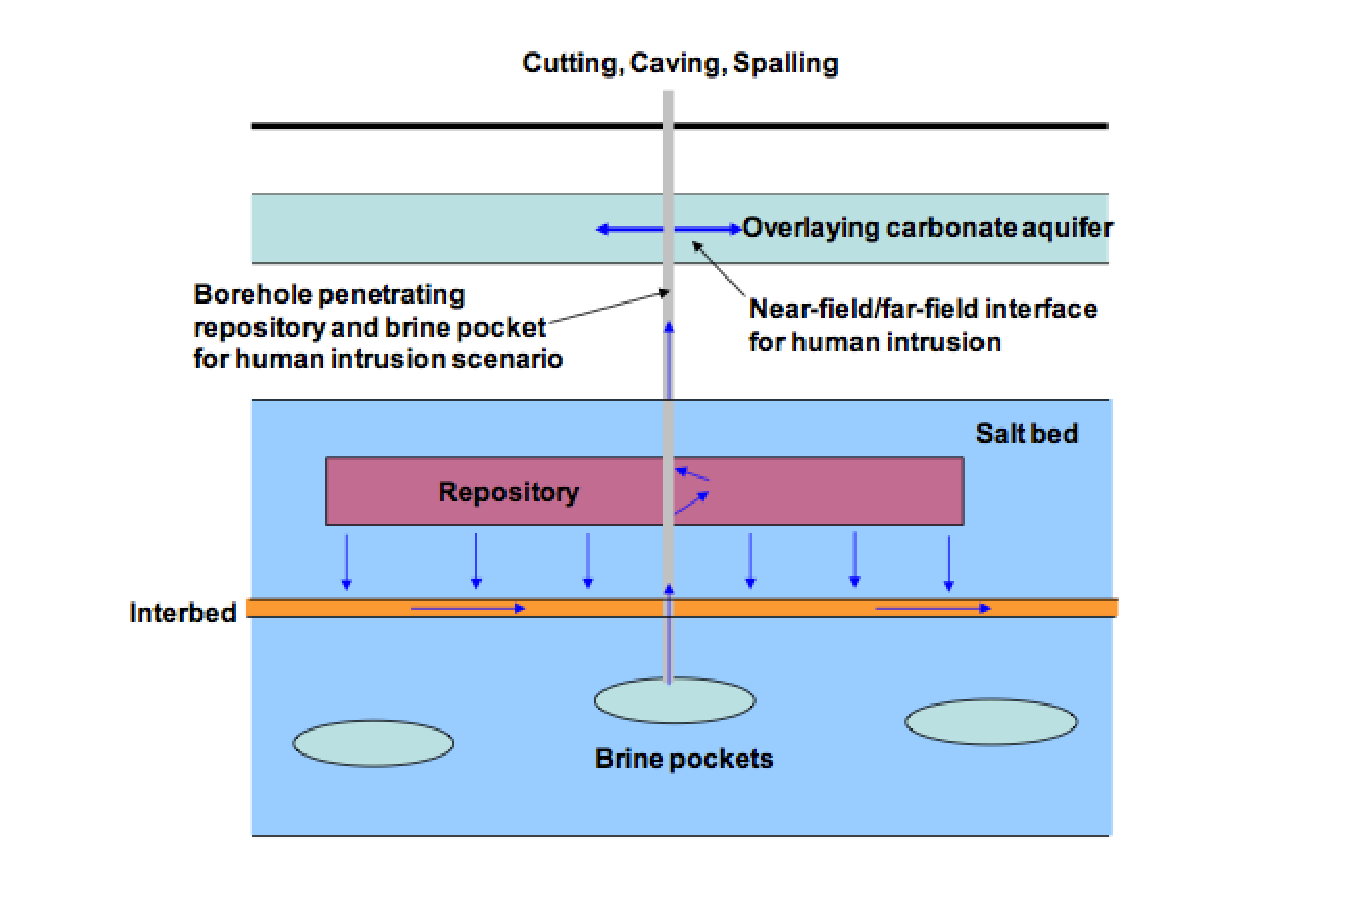
\includegraphics[height=.7\textheight]{./images/saltGPAM.eps}
    \end{center}
    \caption{DOE-NE Used Fuel Disposition Campaign  concept in 
    Salt \cite{clayton_generic_2011}.}
    \label{fig:saltGPAM}
  \end{figure}

\end{frame}

\begin{frame}[c]
  \frametitle{Deep Borehole Disposal Environment}

  \begin{figure}[h!]
    \begin{center}
      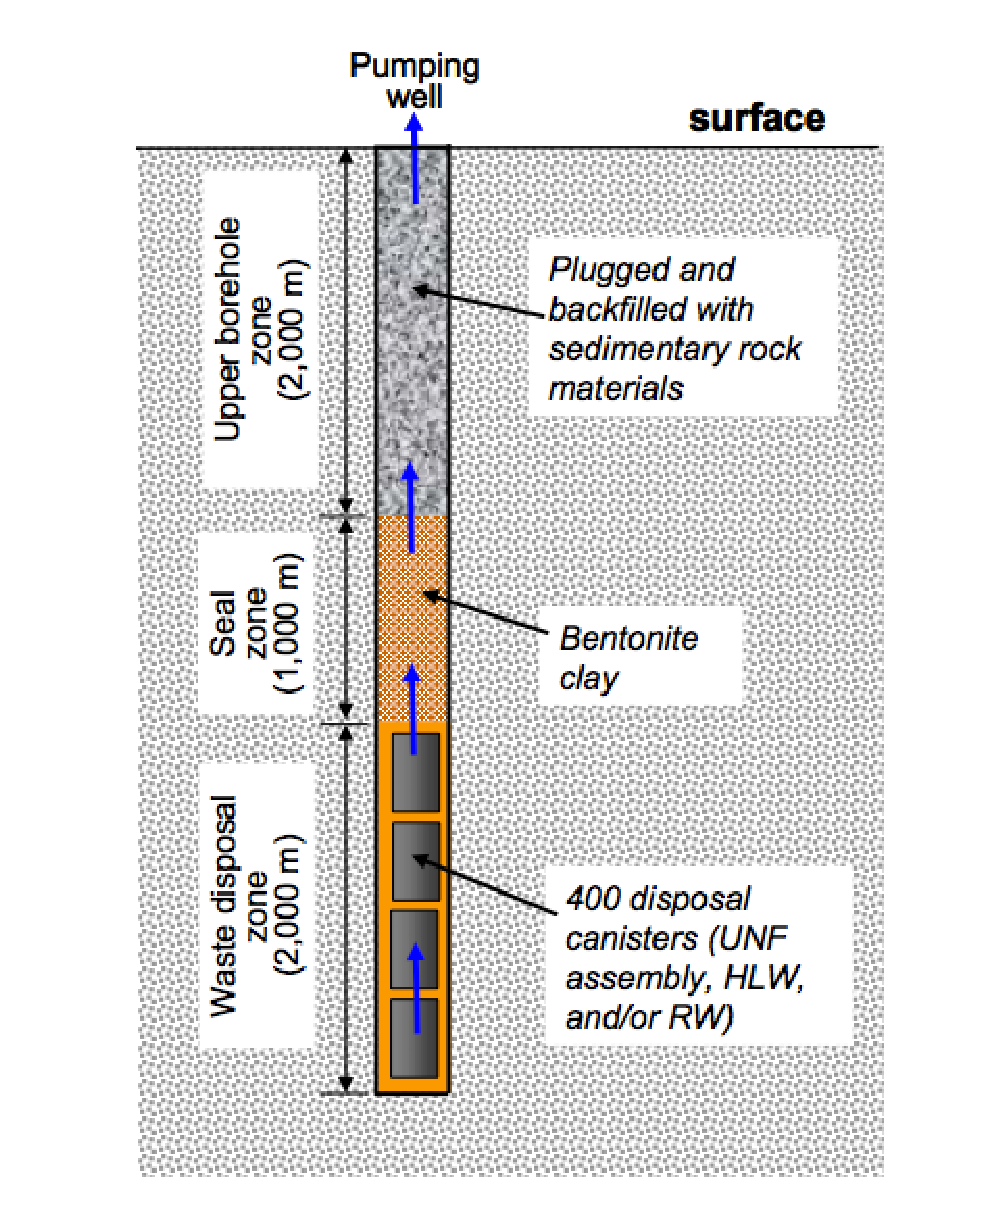
\includegraphics[height=.7\textheight]{./images/boreholeGPAM.eps}
    \end{center}
    \caption{DOE-NE Used Fuel Disposition Campaign Deep Borehole concept 
    \cite{clayton_generic_2011}.}
    \label{fig:boreholeGPAM}
  \end{figure}

\end{frame}


\begin{frame}
  \frametitle{Repository Layouts}

  \begin{minipage}{0.49\textwidth}
    \begin{figure}[h!]
      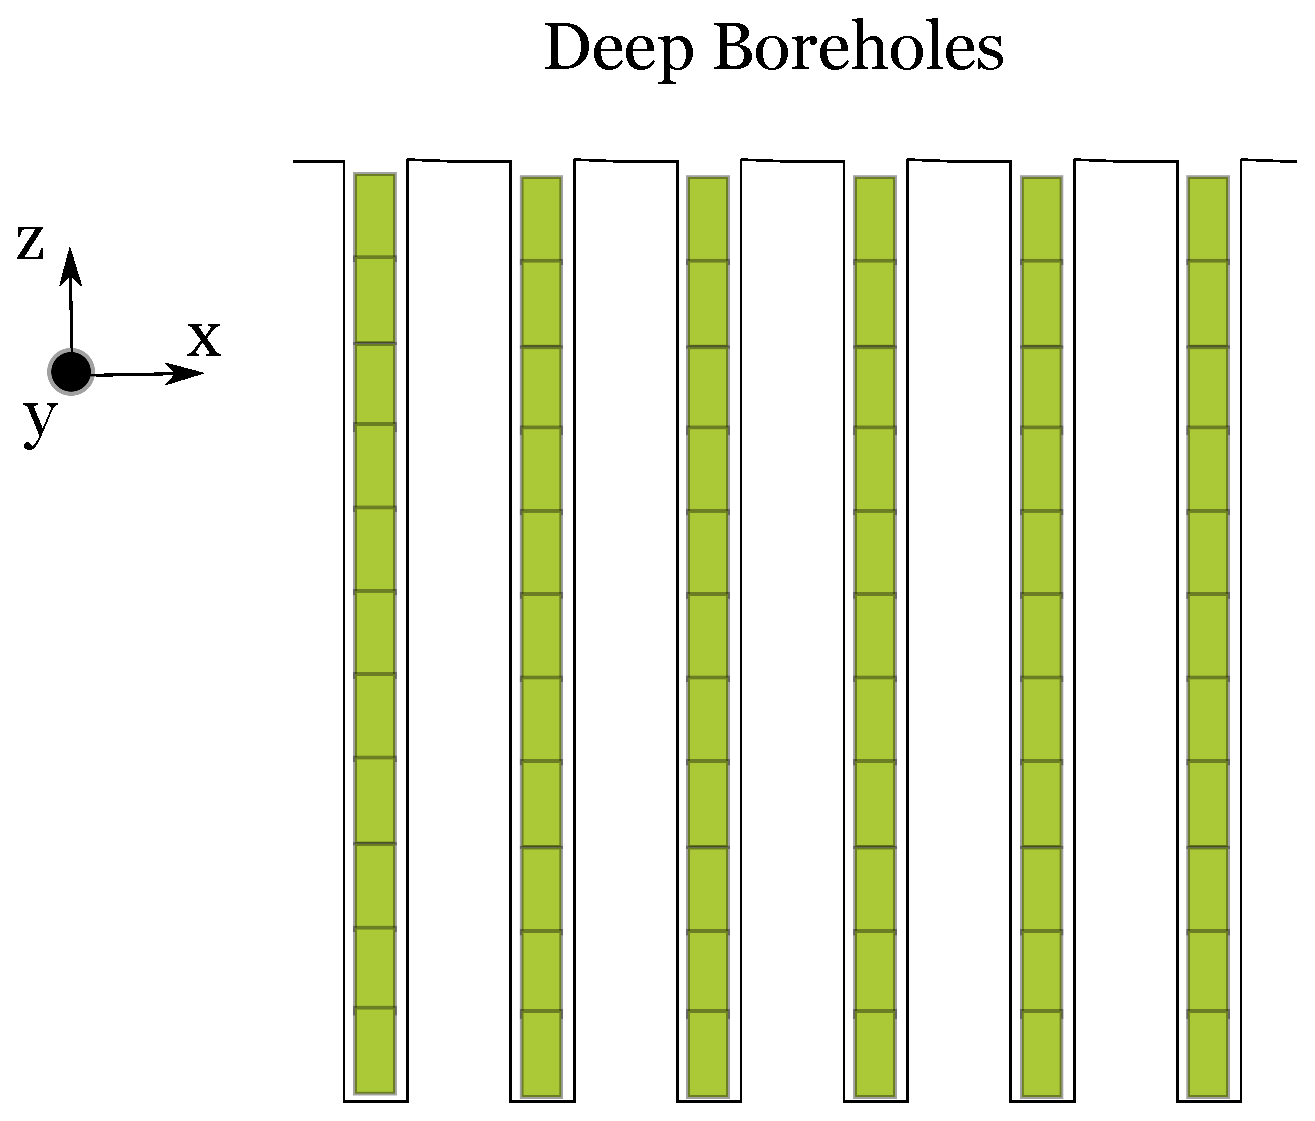
\includegraphics[width=0.75\textwidth]{./images/boreholes.eps}
    \end{figure}
    \begin{figure}[h!]
      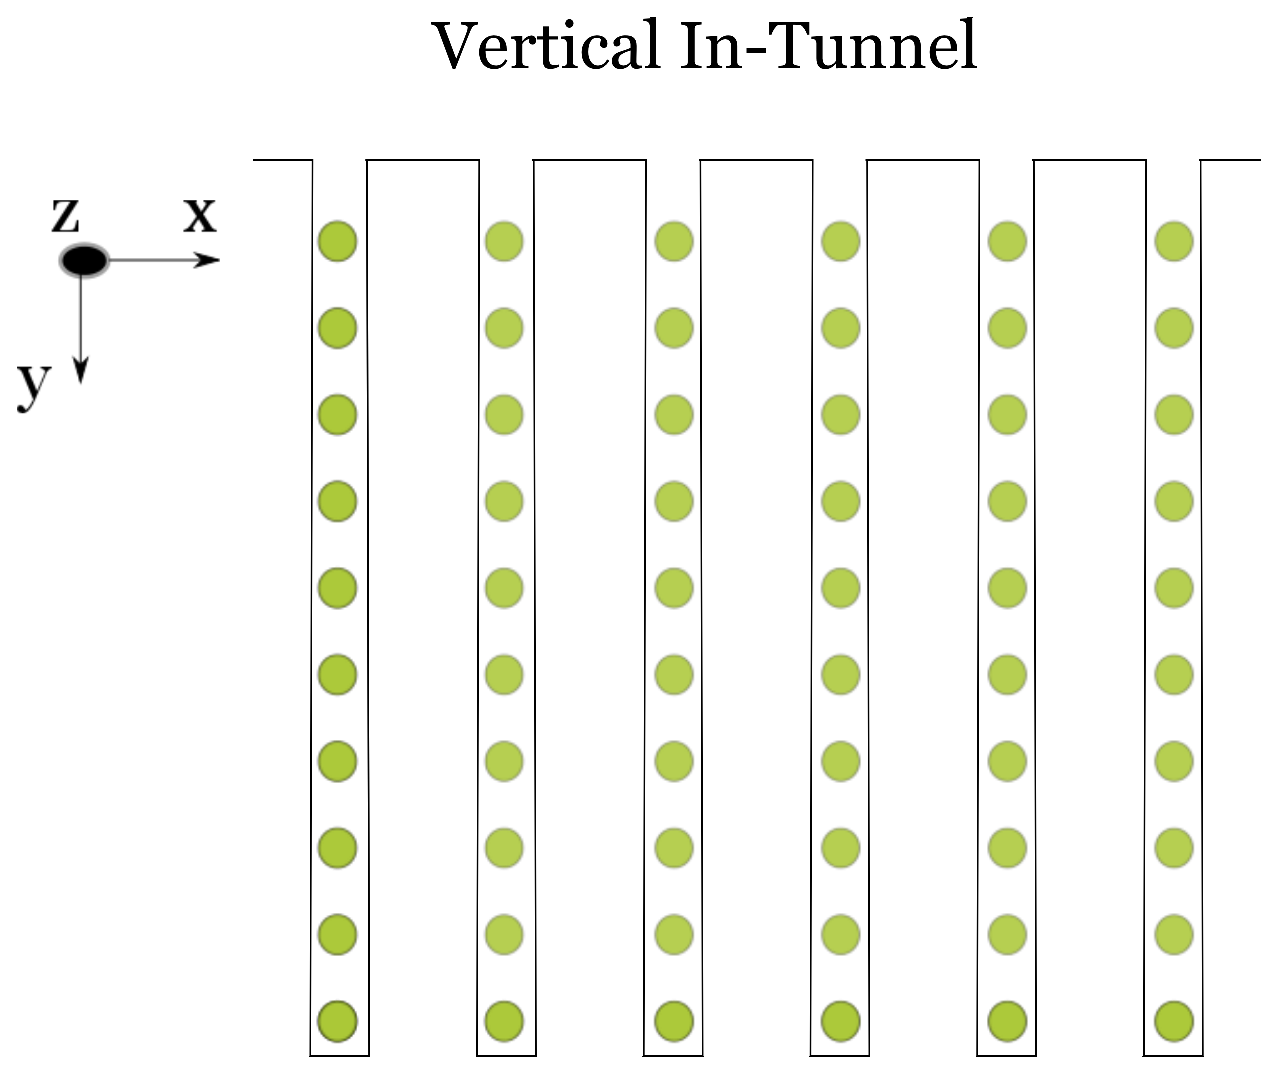
\includegraphics[width=0.75\textwidth]{./images/vertical.eps}
    \end{figure}
  \end{minipage}
  \hspace{0.01cm}
  \begin{minipage}{0.49\textwidth}
    \begin{figure}[h!]
      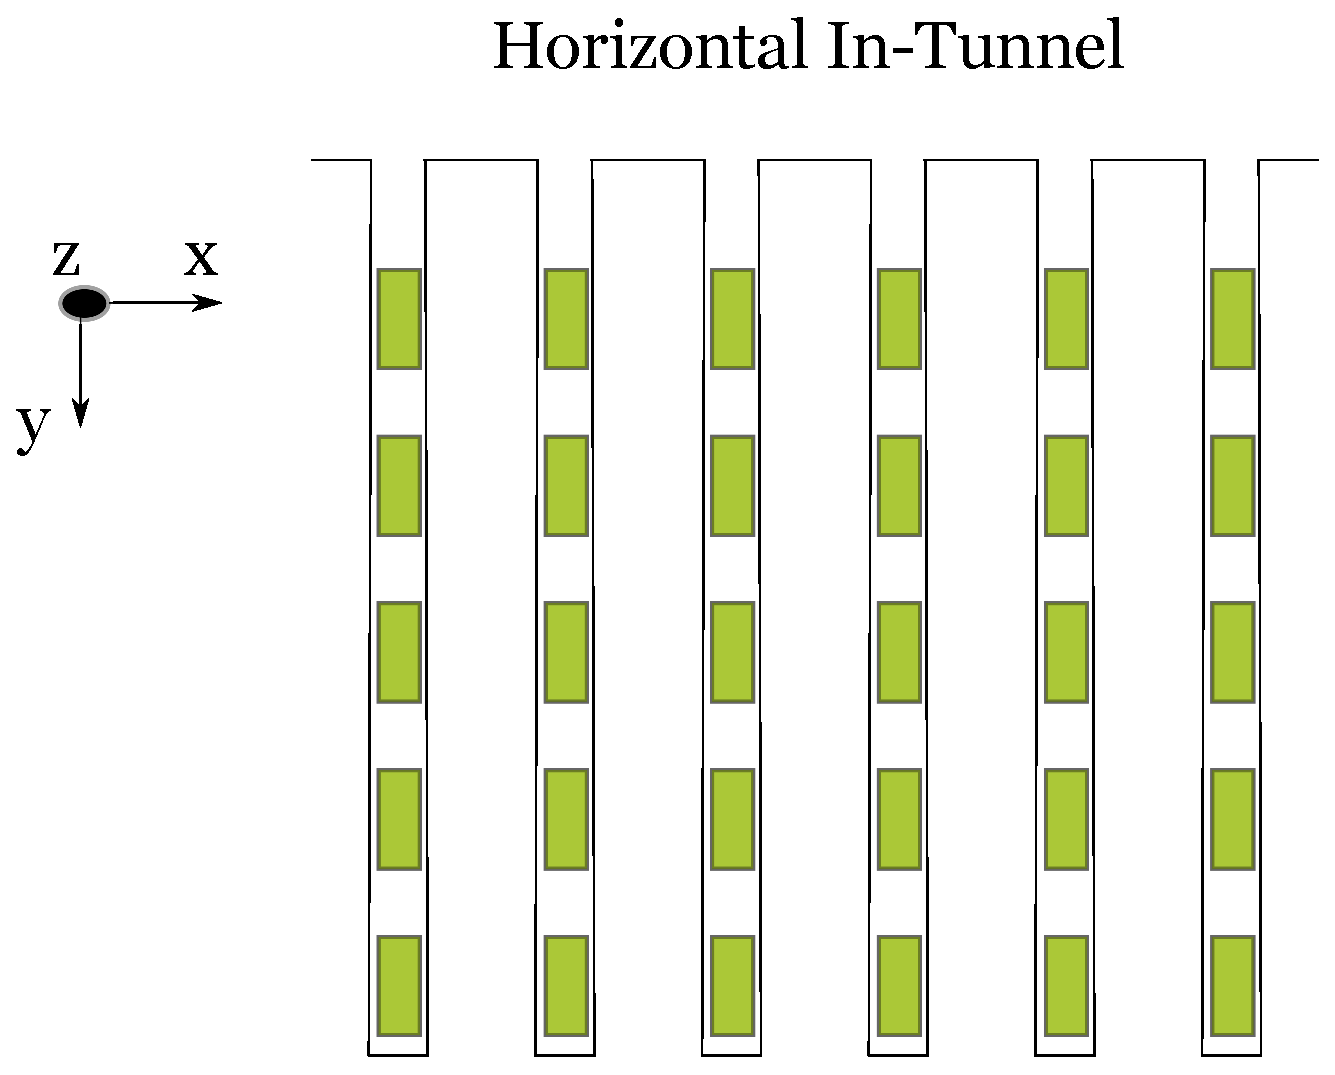
\includegraphics[width=0.8\textwidth]{./images/horizontal.eps}
    \end{figure}
    \begin{figure}[h!]
      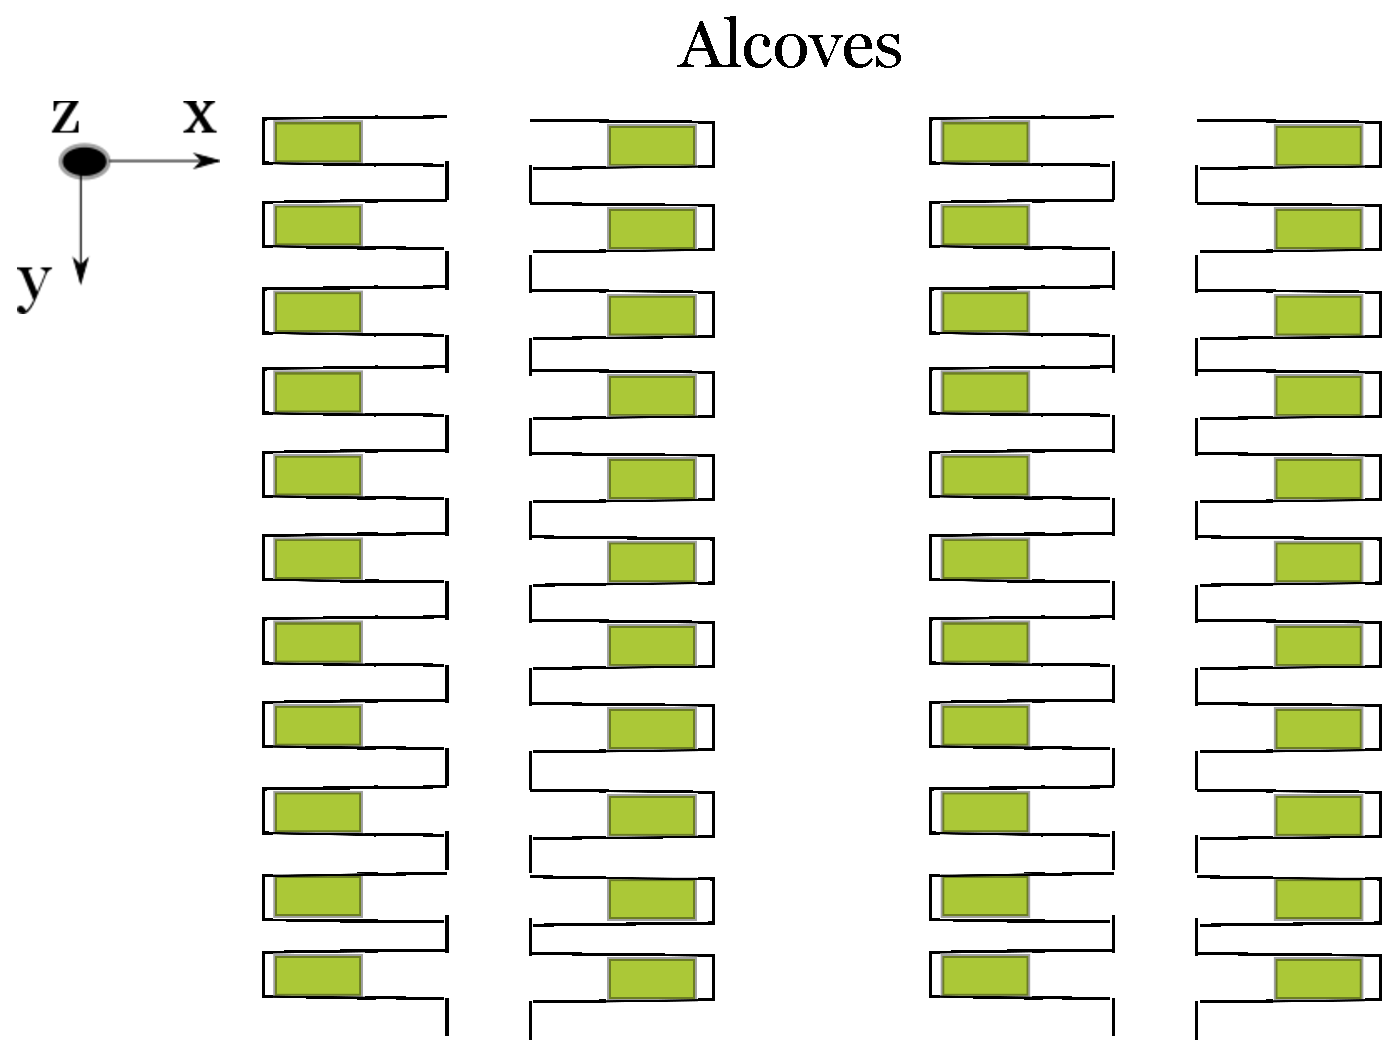
\includegraphics[width=0.8\textwidth]{./images/alcoves.eps}
    \end{figure}
  \end{minipage}

\end{frame}

\begin{frame}[c]
  \frametitle{All Disposal Environments}
  % Table
  %        File: geos_tab.tex
%     Created: Thu Aug 04 11:00 AM 2011 C
% Last Change: Thu Aug 04 11:00 AM 2011 C
%
\begin{table}[h!]
  \centering
  \footnotesize{
  \begin{tabular}{|l|r|r|r|r|}
    \multicolumn{5}{c}{\textbf{Features of Various Concepts}}\\
    \hline
    Feature & Clay & Granite & Salt & Deep Borehole \\ 
    \hline
    \multicolumn{5}{|c|}{\textbf{Hydrology}}\\
    \hline
    Total Porosity $[\%]$    & 34-60  & 0.1 & 0.5 & 0-0.5 \\ 
    Eff. Porosity $[\%]$ & 0.5-5 & 0.0005 & 0.1 & 0.00005-0.01 \\ 
    Conductivity$[m/s]$ & $10^{-11} - 10^{-9}$ & 
    $10^{-6}-10^{-5}$ & $10^{-12}-10^{-10}$ & 
    $10^{-13}-10^{-4}$ \\ 
    Fracturation & none & high & none & low at depth \\ 
    \hline
    \hline
    \multicolumn{5}{|c|}{\textbf{Geochemistry}}\\
    \hline
    Reducing & Near \& Far Field & NF only  & NF only & NF only \\
    Oxidizing & none & Slight in FF & Slight in FF & Slight in FF \\
    Salinity & higher at depth & higher at depth & high & high \\
    pH & $\sim7$ & $\ge7$ & $\ge7$ & $\sim7$ \\
    \hline
    \hline
    \multicolumn{5}{|c|}{\textbf{Design}}\\
    \hline
    Waste Package & Steel, Cu & Steel, Cu & Steel & Steel,Cement \\
    Buffer & -,Fo-Ca,Cement & Fo-Ca,Cement & Crushed Salt & -,Fo-Ca,Cement\\ 
    Depth & 100-500 m & 100-500 m & 100-500m & 3-5km \\ 
    Emplacement & Vert.,Horiz,Alcove & Vert.,Horiz. & Alcove & Vert. \\ 
    Packages/Gallery & one, many & one, many & one, two & 400 \\ 
    \hline
    \hline
    \multicolumn{5}{|c|}{\textbf{Thermal Behavior}}\\
    \hline
    Buffer Limit $[^{\circ}C]$ & 100 (Fo-Ca) & 100 (Fo-Ca) & 180 & 100 (Fo-Ca) \\ 
    Host Limit $[^{\circ}C]$   & 100 (alteration)  & 200 (cracking) & 180 (brines) & none \\ 
    Conductivity $[\frac{W}{m{\cdot}K}]$ & $1-2$ & $2-4$ & $\sim4$  & $2-4$ \\ 
    Coalesence & yes & no & yes & no \\ 
    \hline
  \end{tabular}
  }
  \label{tab:geos_tab}
\end{table}
%  \cite{stober_hydraulic_2006} 

\end{frame}


\section{Methods}
\subsection{Illinois Colors}
\input{fierce}
\section{Conclusion}

%%----------------------------------------%%
\begin{frame}
  \frametitle{Conclusion}
  Thanks!

  Feel welcome to ask any additional questions. \\
  my e-mail address: mmunk2@illinois.edu
\end{frame}

\begin{frame}
  \frametitle{Acknowledgements}
  My work is supported by \ldots  
\end{frame}

%%--------------------------------%%
%%--------------------------------%%
\begin{frame}[allowframebreaks]
  \frametitle{References}
  \bibliographystyle{plain}
  {\footnotesize \bibliography{2017-09-21-anl.bib} }

\end{frame}

%%--------------------------------%%


\end{document}



